% capitulo1.tex
\chapter{Introducción}
\section{Historia de los medios}
%Introducción nueva
%¿Qué son las redes de sensores inalámbricos?
Tomando en cuenta que desde sus inicios la reproducción de medios siempre ha estado relacionada con los últimos avances científicos, los medios de distribución actuales tienen sus bases en los avances que datan  del siglo XIX.\\
Inicialmente los registros de audio con posibilidades de distribución aparecieron con el invento basado del fonógrafo de Thomas Alva Edison, el Gramófono de Emile Berliner, aparecido en 1887 y patentado en 1888. La diferencia con diseño original de Edison está en el medio de registro de audio con el disco de vinilo. Cabe recordar la famosa imagen de la compañía RCA Víctor del Perro escuchando la voz del amo.\\

Análogamente el registro de imágenes en movimiento apareció gracias al cinematógrafo, invento del francés Léon Bouly, y más tarde desarrollado y popularizado por los hermanos Auguste y Louis Lumière, el cual permite la grabación y reproducción del contenido con la misma máquina.\\

Esta tecnología sienta bases para la transmisión de contenidos a gran escala, broadcasting. Para el siglo XX, los avances en tecnología permiten experimentar con difusión a través del espectro de frecuencias.\\

 En los años 1920’s la radio es el medio más popular, llegando a estar presente en 40 millones de hogares estadounidenses, para dos décadas después (1950’s) ser reemplazada en popularidad por la naciente televisión.\\

	Estos medios comunicativos para la década actual (2010’s) mantienen su esencia, que es la transmisión del video y/o audio a una gran cantidad de personas. Si bien el medio por el que se transmite, la resolución, fidelidad y formato han cambiado, las bases son las mismas.\\
	
En la actualidad las transmisiones de audio y video se encuentran en un estado de transición desde medios de comunicación análogo como, por ejemplo, la radio FM, AM y la televisión PAL, NTSC, SECAM, a transmisiones digitales. El motivo de este cambio tecnológico es aprovechar de mejor manera el espectro radioeléctrico, enviando la misma o mayor información que por transmisiones análogas, pero utilizando menos recursos del espectro (Subtel Chile \cite{sota:subtel}).\\

Otro medio de transmisión que ha tomado gran significancia en la última década es la Internet. A través de transmisiones de flujos de datos (streaming), es posible escuchar radios online, ver videos en YouTube, o utilizar servicios de películas “on-demand” como Netflix, por dar ejemplos disponibles en Chile. Todo esto siendo recibido en un computador u otro dispositivo que presente conectividad a la red.\\

Estos dispositivos alternativos tienen el peso de llevar la recepción de medios audiovisuales por un nuevo rumbo y ya están siendo considerados por las empresas que generan el contenido, al proveer salidas directas a televisores con Internet; consolas de videojuegos con navegador web o aplicaciones cliente para servicios de audio o video on-demand. Otro punto a tener en cuenta es la mayor importancia que tiene el crecimiento del consumo de dispositivos móviles como celulares o reproductores portátiles multimedia, donde se puede llegar a una audiencia aun más grande.\\

\clearpage
\section{Tecnología actual relacionada}

\subsection{Estado actual de las transmisiones}

Considerando que el objetivo de este trabajo tiene relación con la distribución y recepción de contenidos audiovisuales. Se presentan distintos medios funcionando actualmente.\\

Video-on-demand: es un servicio de distribución que permite a los usuarios seleccionar y ver o escuchar el contenido de video o audio de manera personalizada, ofreciendo la opción de solicitar el contenido en el momento exacto que lo desee.  La plataforma para poder reproducir el contenido se puede encontrar implementada como aplicación en un computador o a través de un dispositivo con conexión directa a al televisor y al proveedor del servicio. En Chile este servicio es provisto por la compañía VTR a través de su dispositivo D-Box, este dispositivo cumple además la función de DVR.\\

La compañía Netflix también provee este servicio, sin embargo el medio de transmisión es Internet, ofreciendo a sus clientes suscripciones que permiten el acceso al catalogo de películas.\\

En Chile se ha posicionado a partir de Septiembre de 2011, y considerando simplificar registro de nuevos usuarios, su potencial acogida nuevo usuarios se magnifica al poner a disposición de sus clientes el acceso a los contenidos a través de variadas plataformas de reproducción, como consolas de videojuegos de sobremesa, Nintendo Wii, y PlayStation 3, consolas portátiles como Nintendo 3DS, acceso vía web y aplicaciones para televisores con InternetTV. \\

Podcast: es una serie de archivos de medios digitales (audio o video) lanzados en forma periódica por episodios, este sistema permite al usuario descargar el contenido de su interés para poder verlo o escucharlo más tarde.\\

El modo de distribución se diferencia de otras formas de transferencia de internet como lo son la descarga directa al estar todos los archivos catalogados en un servidor central, este además provee a los usuarios una vía de distribución a través de RSS Feeds, que son archivos de información en XML (extended markup language) diseñados para compartir actualizaciones de sitios web, popularizados por los blogs.\\ 
El uso de RSS Feed para los podcast permite informar a las personas suscritas de nuevos contenidos, aunque no es necesario que la persona esté suscrita para obtener alguna información en especifico. 
Su uso se ha popularizado por la plataforma iTunes desarrollada por Apple, que en su versión 4.9 de 2005, abrió a una gran base de usuarios este nuevo medio de comunicación. No solo se utiliza para entregar programas de radio, sino que también documentos y programas de televisión, de manera gratuita.\\

Streaming media: este método provee constantemente datos multimedia al usuario final, que reproduce mientras tanto el servidor se encuentra entregando la información.
El nombre se refiere a que el método de entrega es continuo, sin interrupción, debido a que los datos recibidos se almacenan en un buffer de memoria que se va liberando mientas se reproduce. Es decir los datos de audio o video, no son descargados,  es un acceso directo al contenido intangible.
Un uso más reciente que se le ha dado al método streaming es lo que se llama LiveStreaming, donde el contenido a distribuir es capturado en el momento, una tranmision en vivo que es posible de ser recibida por el usuario casi al momento que ocurre gracias al flujo o stream de datos.
La base fundamental de este método de distribución, es la utilización de protocolos ligeros de la capa de transporte, como lo es UDP (User Datagram Protocol) que a diferencia del protocolo TCP (Transmission Control Protocol), no asegura la entrega en caso de fallo, permitiendo obviar los paquetes, priorizando la continuidad del flujo en el tiempo sobre la fiabilidad de los contenidos.  En la capa de aplicación se ha desarrollado un protocolo con este objetivo, toma como base la conexión mediante UDP para realizar el enlace, es llamado Real-time Transport Protocol (RTP \cite{sota:rtp-draft}).\\

Aun así existe un protocolo de la capa de aplicación que utiliza TCP para realizar el enlace. Este fue desarrollado originalmente por Macromedia, siendo ahora propietario Adobe Systems, el Real Time Messaging Protocol (RTMP \cite{bib:rtmp-specs}) fue desarrollado para realizar streaming multimedia a través de TCP con baja latencia, esto lo logra gracias al envío de la mayor cantidad de información por enlace. \\
	
	De esta metodología Apple Inc. ha desarrollado un nuevo método llamado HTTP Live Streaming, que se diferencia al utilizar pedazos de audio o video  ordenados en una lista de reproducción de extensión m3u que es actualizada a medida que nuevos contenidos son creados. A diferencia del streaming nombrado anteriormente, este flujo de datos se trasmite a través del protocolo HTTP (Hypertext Transfer Protocol \cite{sota:rfc-http}), el cual es de una capa superior (de aplicación) posibilitando la transferencia de los datos multimedia con un servidor web ordinario como por ejemplo Apache. Además posibilita la transmisión en redes donde firewalls o proxies bloqueen contenido ya que se enmascara como trafico de hipertexto.

\subsection{Almacenamiento del Contenido}

Otra tecnología que está relacionada con este tema, tiene que ver con la toma de registro de los medios recibidos. Existen en la actualidad los llamados DVR (digital video recorders), dispositivos interactivos que cumplen con la grabación de la señal de televisión o video, siendo almacenada en formato digital.\\

 Esta información queda guardada en el disco duro o memoria del sistema, para poder ser vista después. A diferencia de una antigua videograbadora, el medio de almacenamiento y el formato es digital, permitiendo tomar registro y así manipularlo mediante software.\\
 
	El concepto es aplicado en hardware para televisión e implementado en decodificadores de televisión pagada. En el caso de proveedores de cable, la transmisión es recibida por el enlace coaxial, donde el dispositivo cumple la función de decodificar la señal digital y almacenarla si posee características de DVR.

\subsection{Registros de Stream}

Se puede implementar este concepto de DVR en software de computadores de escritorio, desarrollando alguna aplicación que permita registrar los segmentos transmitidos por streaming para ser reproducidos en otra ocasión. \\

	Servicios de streaming bien populares como Justin.TV, UStream o Twittcam permiten transmitir video a través de sus plataformas web, y permiten la revisión del contenido tiempo después que este ha finalizado. En cierta parte este comportamiento se asemeja al DVR, pero no posibilita moverse en el tiempo mientras se transmite.\\

En Chile, se ha desarrollado una aplicación más sofisticada por parte de la empresa AltaVoz S.A. con su producto SocialStream, el cual permite retroceder y revisar el contenido mientras la transmisión se encuentra en curso. Este registro es encargado al servidor quien administra los pedazos de información multimedia, una aplicación cliente entabla conexión para realizar pedidos de la información en el tiempo que desea el usuario.
Esta característica lleva como nombre comercial TimeShift.

\section{Propuesta de Proyecto}
\subsection{El Smartphone}
Primero que todo se debe definir el concepto de Smartphone, lo cual es un teléfono portátil con conectividad a las redes celulares y que presenta características adicionales respecto a los teléfonos móviles comunes.\\

Sus bases se sientan en los siguientes conceptos:
\begin{itemize}
\item Su funcionalidad puede ser extendida a través de aplicaciones adicionales.
\item Debe poseer un teclado QWERTY físico o virtual.
\item Debe permitir estar siempre conectado a la Internet.
\end{itemize}
Considerando estos conceptos se puede encasillar como Smartphone a los teléfonos Blackberry, iPhone y Android.

\subsection{Trasfondo}
La mayoría de los smartphones permiten el acceso a internet a través de la red celular utilizando distintas tecnologías de transmisión de datos (no sólo WiFi), como los son actualmente EDGE y 3G. Estas se encuentran en incesante desarrollo, presentando mejoras en la velocidad de transferencia de datos.\\

La constante mejoría en la velocidad de transmisión en redes celulares ha permitido la reproducción de contenidos multimedia. Un avance similar a lo experimentado en la década de 1990 por los computadores multimedia de escritorio. En primera instancia con aplicaciones con contenido audiovisual (imagen, audio, video, texto) ejecutadas localmente, para luego llegar a recibir y transmitir este contenido a través de la world wide web.\\

Los smartphones actuales ejecutan sistemas operativos avanzados que proveen módulos de conexión  a redes, ya sea celular, WiFi, o Bluetooth, si es que el hardware lo incorpora. Además de navegadores web diseñados especialmente para estos dispositivos, con características como presentar en pantalla reducida o ajustada a la resolución, interfaz táctil, teclado numérico, etc.\\

Considerando estas 2 bases, conectividad y sistema operativo capaz, es posible implementar una aplicación que se asemeje a la experiencia en computadores de escritorio.\\

\subsection{La Problemática}
Actualmente se encuentra en desarrollo en Chile el producto SocialStream, para computadores de escritorio y aparatos de sobremesa. 
Una herramienta que permite registrar en el momento, una transmisión en vivo, ya sea de audio o video. Posibilitando al consumidor del contenido, retroceder a un punto en específico, pausar  y avanzar (limitado por el punto más reciente de la transmisión). 
A diferencia de dispositivos de sobremesa (set top boxes) como lo son TiVo u otros DVR, el registro de la transmisión es encargado al servidor que provee los contenidos a los clientes que se conectan, y esto contenidos no son guardados localmente.
Este sistema nos significan los siguientes beneficios: 
\begin{itemize}
\item Ahorro para el consumidor, espacio en sus dispositivos de almacenamiento
\item Cierto control del proveedor sobre la distribución  y copia de los contenidos
\item La posibilidad de portar a otras plataformas como consolas de videojuegos o dispositivos móviles.
\end{itemize}

Las bases de esta herramienta se fundan sobre Adobe Flash gracias a su protocolo RTMP. Y considerando el estado actual de las relaciones entre Apple y Adobe (carta de Steve Jobs, exCEO de Apple) surge nuestro principal problema:

\begin{itemize}
\item Las aplicaciones que cumplen la función de reproducción de los contenidos están desarrolladas en el lenguaje de programación ActionScript, propio de Adobe.
\item En las plataformas de escritorio y algunos smartphones, esto no significa un problema. Sin embargo los dispositivos de Apple con el sistema operativo iOS no presentan compatibilidad con estas tecnologías Flash.
\end{itemize}

	En las siguientes figuras \ref{sshot_Android_sstream} y \ref{sshot_iOS_sstream} se puede notar claramente el problema que genera en iOS la falta de soporte de tecnologías Adobe.

%\clearpage 
\begin{figure}[h!]
	\centering
	% \fbox{ } % la encierra en un cuadrado, sirve para código también
	 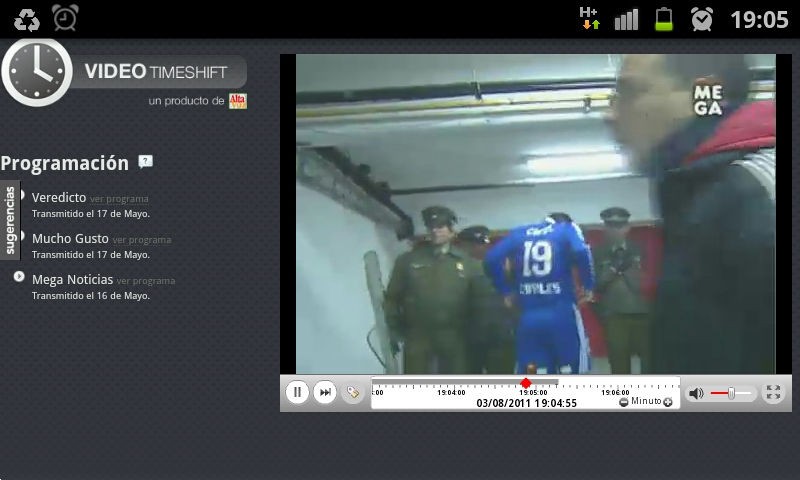
\includegraphics[scale=0.47]{imgs/sshot_Android_sstream.jpg}
 	\caption{Reproducción de SocialStream en Android OS.}
	\label{sshot_Android_sstream}
\end{figure}
%\vspace{3cm}
\begin{figure}[h!]
	\centering
	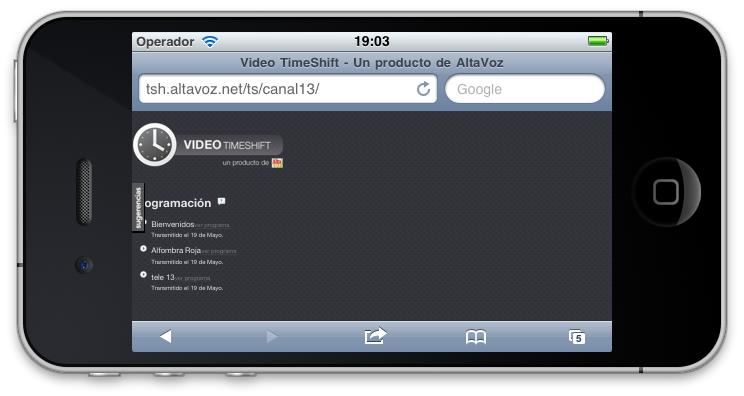
\includegraphics[scale=0.55]{imgs/sshot_iOS_sstream.png}
	\caption{Reproducción de SocialStream en iOS}
	\label{sshot_iOS_sstream}
\end{figure}

\newpage
\subsection{Posibles Soluciones}

A la fecha, las herramientas de distribución de audio y/o video por streaming, están limitadas a los reproductores provistos por la interfaz de programación de aplicaciones (API) de iOS. En donde al reproducir contenido por streaming presentan la opción de retroceder la cantidad de  tiempo almacenada en el buffer de datos. \\

%\clearpage
\begin{figure}[h!]
	\centering
	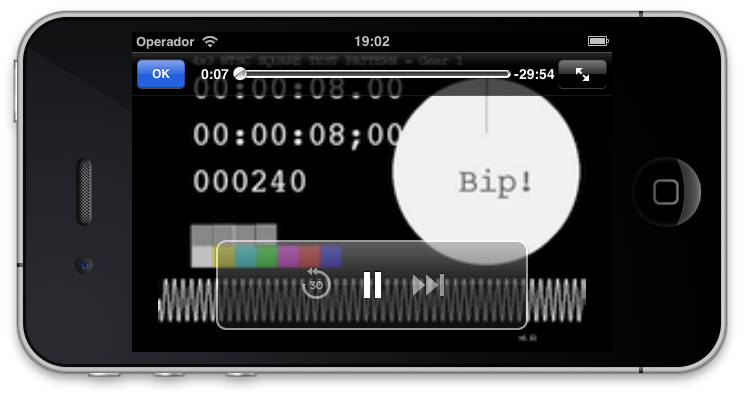
\includegraphics[scale=0.55]{imgs/sshot_iOS_hls.png}
	\caption{Reproducción de flujo video por HTTP Live Streaming}
	\label{sshot_iOS_hls}	
\end{figure}

De la figura \ref{sshot_iOS_hls} se puede notar el botón a la izquierda en la barra inferior de  la pantalla, este hace retroceder en 30 segundos la reproducción.\\

Esta característica es propia del framework MediaPlayer. que simplifica de gran manera la necesidad de mostrar video en el dispositivo. Este uso también se puede aplicar para la reproducción  de  audio y video.
Se debe dejar claro que Apple es sumamente restrictivo en el uso de la API de iOS. \\
Para el desarrollo de aplicaciones, estas deben utilizar solo llamadas al sistema que estén indicadas en sus documentos guía, por lo tanto una vía para desarrollar una solución de reproductor que provea la posibilidad de saltar en la línea del tiempo de reproducción sin importar que tan larga sea la transmisión en vivo, depende de las bases MediaPlayer. \\

En la documentación actual de iOS v4.3 se encuentra AVPlayer (audio video player) [link] que pone a disposición las llamadas y manejo de datos de audio y/o video.


\subsection{Soluciones actuales}
En computadores de escritorio, existen reproductores hechos en Flash que permiten la reproducción de transmisiones de streams en vivo de video FLV y audio en AAC.\\

	En el caso de smartphones, solamente el sistema operativo Android permite mostrar contenido Flash destinado a computadores de escritorio. Por lo tanto la reproducción de videos en formato FLV y audio AAC está asegurada gracias a la carga del reproductor programado para ese propósito.\\

A la fecha (septiembre de 2011) se encuentra en desarrollo una salida de datos del servodor de medios Wowza, esta salida está basada en la tecnología HTTP Live Streaming, sistema impulsado por Apple para la transmisión de audio y video a través del protocolo de transferencia de hipertexto. Esta característica de Wowza permite reproducir video con  saltos en el tiempo y al no utilizar el encapsulado FLV, es compatible con las tecnologías de iOS.

\subsection{Pros y Contras de una nueva solución}
En el caso de la salida con HTTP Live Streaming de Wowza, se puede considerar como punto en contra la interfaz gráfica que no se adecua para el control de la transmisión en caso que esta sea muy amplia. Otro punto en contra es que esta solución tiene un costo monetario por licencias de transmisión.\\

	También se puede tomar como punto en contra que la salida de HTTP Live Streaming es reproducida por el MPMediaPlayer estándar, sin mucha versatilidad para caracteristas expansivas, como por ejemplo integrar redes sociales como twitter o facebook en para comentarios.\\

	En el caso de otros smartphones y sistemas operativos, la reproducción del stream de datos está permitida si es que el sistema operativo soporta Adobe Flash.\\

	Un punto en contra de Android es la variabilidad del hardware que corre dicho sistema operativo. Existiendo distintos modelos y versiones de un Smartphone compatible con él, estos pueden o no presentar los contenidos de forma correcta, por ejemplo dispositivos con procesadores (CPU) de uno o múltiples núcleos, o también la incorporación de procesadores gráficos (GPU) que permiten la decodificación del video por hardware.\\

En el caso de los dispositivos iOS, todos estos son diseñados y construidos por Apple Inc., siguiendo un estándar que permite una experiencia similar en los distintos productos.

\subsection{El beneficio de llegar a nuevas audiencias}
Se debe tomar en cuenta que los dispositivos iOS, entiéndanse iPhone, iPad y iPod Touch; representan una gran participación en cada uno de sus mercados: smartphones, tablet-pc y reproductores  multimedia, respectivamente. Donde su fuerte y enfoque principal es el mercado de smartphones (ver Tabla 2), llegando muy cerca al líder Android de Google 43,4\% que abarca una gran cantidad de fabricantes de hardware, si se toma en cuenta que Apple Inc. Es el único fabricante del iPhone, su 18,2\% de participación es significante.\\

iPad actualmente domina el mercado con un 68\% de participación, en el área de computadores tipo tablilla (tablet-pc), debido a que este producto trajo la innovación y la pauta de diseño para sus competidores, que aun no logran igualar la experiencia para el usuario con versiones modificadas de Android, mientras que iOS toma sus bases en el ya consolidado Mac OS X.\\

En el caso de los reproductores multimedia, la popularidad de los dispositivos iPod desde los principios de la década de 2000, ha facilitado la adopción de la línea más reciente que también corre iOS.\\

Tomando en cuenta los puntos indicados anteriormente, se deduce que no son dispositivos que se deben obviar. Al no poseer una aplicación compatible con el sistema de distribución de contenidos, se está acotando en gran parte a la audiencia.\\

En resumen, estos puntos ayudan a presentar que es viable un reproductor alternativo, ya sea como aplicación o biblioteca de desarrollo para nuevos proyectos. \\


%¿Cuáles son las áreas de investigación y desarrollo de WSN?
%buscar como continuar después de una itemezación con dos puntos y separados por comas.

%Presentar el tema del ruteo y recolección de datos

%IR DE LO GENERAL A LO PARTICULAR!
%El capítulo de introducción debe comenzar explicando que son las 	WSNs.
	%\section{Redes de sensores inalámbricos}
	
	%\section{Aplicaciones}
%En el mundo

%En Chile

	%\section{Protocolo de ruteo para un sistema de recolección de datos}
	%\section{Visión general de los requerimientos}
%Hablar de la aplicación objetivo y cuáles son sus requerimientos 

%Títulos alternativos
% El objetivo de este trabajo es implementar un protocolo de ruteo multihop como parte de un sistema de recolección de datos que está construido sobre una red de sensores inalámbricos. Este sistema está orientado principalmente al monitoreo de variables físicas principalmente relacionadas con la agricultura, como la humedad y la temperatura de los suelos, en zonas de difícil acceso y que no cuentan con redes de distribución eléctrica.

%En el marco de este trabajo, los objetivos generales son los siguientes:
%\begin{enumerate}
%  \item Informar sobre los protocolos de ruteo de mensajes para redes de sensores inalámbricos.
%  \item Desarrollar una red de sensores inalámbricos, utilizando la plataforma de hardware TmoteSky.
%  \item Desarrollar una aplicación para la recolección de datos de la red.
%  \item Evaluar el consumo energético de la red implementada.
%\end{enumerate}

% El primer objetivo se desarrolla en profundidad en el capítulo 2. El segundo objetivo se desarrolla en los capítulos 3, 4 y 5, donde se plantea un diseño de protocolo y posteriormente como se implementa éste. El tercer objetivo se desarrolla en los capítulos 3 y 5 como parte de las verificaciones del sistema. Finalmente, en el capítulo 5 se evalúa el consumo energético el protocolo.\\
 
	%\section{Estado del Arte}


%\subsection{Protocolo de ruteo}
%\begin{figure}[H]
 %\centering
 %\includegraphics[scale=0.8]{imgs/PilaModeloOSI.eps}
 %\caption{Pila de red establecida por el Modelo OSI}
%\end{figure}

	% \subsection{Algoritmos de ruteo propuestos en la literatura}

%En esta sección debería dar una breve reseña  de cada protocolo, con sus referencias.
	%\subsection{Protocolos implementados}

	%\subsection{Hardware de desarrollo}
%De lo general a lo particular
% Qué tipo de hardware existe?

%Debo incluir info sobre los motes que soportan tinyos
	% \subsubsection{Plataformas TinyOS}
	%\subsubsection{Plataformas Zigbee}
	
%Debo incluir info sobre los motes que soportan Zigbee, simpliciti.
	% \subsubsection{Otras plataformas}
	%\subsection{Software para redes de sensores inalámbricos}

%TinyOS, ZStack, SimpliciTI, etc
%Breve descripción de tinyOS e indicación para revisar el anexo XX.
	%\subsubsection{TinyOS}
	%\subsubsection{Contiki}

%Breve descripción de ZStack, basarse en pagina de ti del zstack
	%\subsubsection{Z-Stack}

%Breve descripción de SimpliciTI, basarse en pagina de ti de simpliciti
	% \subsubsection{SimpliciTI}

%Breve descripción de la de los sunspots, basarse en documentacion
	%\subsubsection{Java y SunSpot}

%Breve descripción de alguna otra de otro fabricante..freescale o atmel.

